\subsubsection{Part A}
		Using the circuit shown in figure \ref{fig:circuit1}, we measured the drain current with $V_{bs} = 0 V$, $V_{gs} = 2.5 V$, and $0V \le V_{ds} \le 5 V$.
		\FloatBarrier

		\begin{figure}[h!]
		\centering
		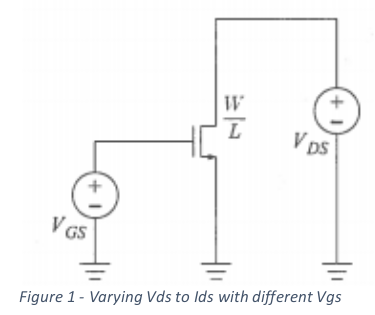
\includegraphics[scale=0.75]{./images/circuit1.png}
		\caption{The circuit tested in part 1.}
		\label{fig:circuit1}
		\end{figure}

		\FloatBarrier
		From the data collected for $I_{ds}$ and $V_{ds}$, the NMOS starts in triode mode. 
		A dramatic increase in drain current is observed in this region.
		This increase begins to taper off around $V_{ds}\approx0.8V$, as the NMOS enters saturation mode. 
		The threshold voltage is approximated to be $V_{tn} = 1.7 V$.

		\begin{equation}
		\label{eq:threshold}
		V_{tn} = V_{gs} - V_{ds} = 2.5 V - 0.8 V = 1.7 V
		\end{equation}

		\FloatBarrier

		\begin{figure}[h!]
		\centering
		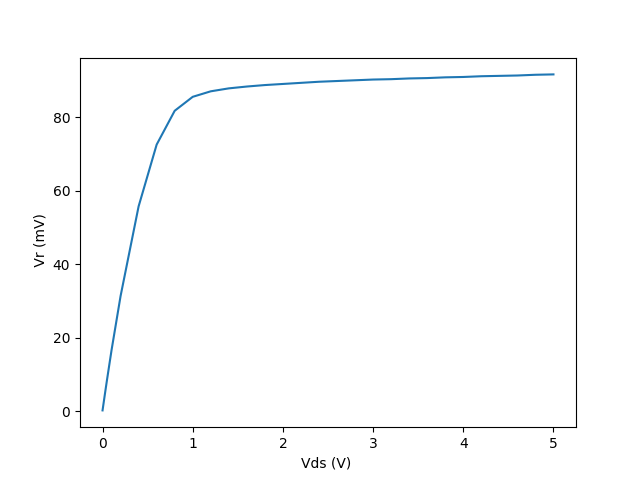
\includegraphics[scale=0.75]{./data/nmos.png}
		\caption{The resulting $I_{ds}$ vs $V_{ds}$ graph for $V_{gs}=2.5V$.}
		\label{fig:nmos}
		\end{figure}

		\FloatBarrier
		During testing, capacitive effects in the triode region are observed. 
		Increasing the drain voltage past $V_{ds}=0.15V$ results in $I_{ds}\approx 166 \mu A$.
		However, decreasing the drain voltage afterward to $V_{ds}=0.15 V$ produces $I_{ds}\approx 310 \mu A$.

		\subsubsection{Part B}
		The same parameters from part A are used in part B, except the gate voltage is increased to $V_{gs} = 5V$. 
		From the $I_{ds}$ and $V_{ds}$ curve in figure \ref{fig:nmos_5v}, the NMOS is operating in triode mode for $V_{ds} \le 3.2V$ and saturation otherwise.

		\FloatBarrier

		\begin{figure}[h!]
		\centering
		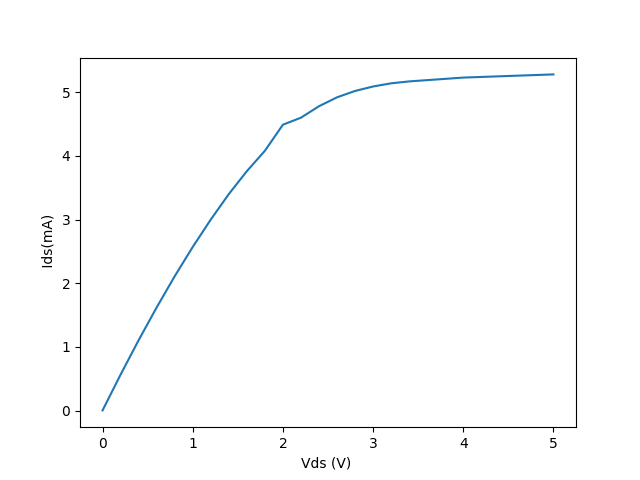
\includegraphics[scale=0.75]{./data/nmos_5v.png}
		\caption{The resulting $I_{ds}$ vs $V_{ds}$ graph for $V_{gs}=5V$.}
		\label{fig:nmos_5v}
		\end{figure}

		\FloatBarrier
		The approximation from part A for the threshold voltage of $V_{tn} = 1.7 V$ can be confirmed.
		
\begin{equation}
	\label{eq:thresh_5V}
		V_{ds} = V_{gs} - V_{tn} = 5 V - 1.7 V = 3.3 V.	
\end{equation}
This result for $V_{ds} = 3.2 V$ as the edge of saturation agrees well with the measured data. 
On the curve, the drain current stays fairly constant after approximately $V_{ds}=3.2 V$.
After comparing the percentage of change in the drain current and drain voltage, it is determined that after $V_{ds} = 3.2 V$ the change in the drain current stays at less than one percent, despite the change in drain voltage of about five percent. 
This result proves that the result of $V_{tn} = 1.7 V$ is a good approximation for the threshold voltage.
